\documentclass[aspectratio=169, 11pt]{beamer}
\usetheme[progressbar=frametitle, numbering=fraction, block=fill]{metropolis}

\usepackage{amsmath, amssymb}
\usepackage{graphicx}
\usepackage{booktabs}
\usepackage{xcolor}
\usepackage{tikz}
\usetikzlibrary{calc, positioning, arrows.meta}
\usepackage{fontawesome5}
\usepackage{hyperref}

% --- Palette: keep it subtle, no rainbow text ---
\definecolor{ocean}{HTML}{1B4F72}
\definecolor{accent}{HTML}{E67E22}

\setbeamercolor{palette primary}{bg=ocean, fg=white}
\setbeamercolor{frametitle}{bg=ocean, fg=white}
\setbeamercolor{progress bar}{fg=accent, bg=ocean!20}
\setbeamercolor{alerted text}{fg=accent}

% Kill hyphenation
\tolerance=1
\emergencystretch=\maxdimen
\hyphenpenalty=10000
\hbadness=10000

% Fonts
\setbeamerfont{title}{size=\large, series=\bfseries}
\setbeamerfont{subtitle}{size=\small}
\setbeamerfont{author}{size=\small}
\setbeamerfont{institute}{size=\scriptsize}
\setbeamerfont{date}{size=\scriptsize}

% Bullet style
\setbeamertemplate{itemize items}[circle]

\title{From Pixels to Patches}
\subtitle{\faSwimmer~Pooling Strategies for Earth Embeddings}
\author{%
  \textnormal{\small
  Isaac Corley\textsuperscript{1} \quad
  Caleb Robinson\textsuperscript{2} \quad
  Inbal Becker-Reshef\textsuperscript{2} \quad
  Juan M. Lavista Ferres\textsuperscript{2}}%
}
\institute{%
  \textsuperscript{1}Wherobots \qquad
  \textsuperscript{2}Microsoft AI for Good Research Lab%
}
\date{ICLR 2026 \enspace\textbar\enspace ML4RS Workshop}

\begin{document}

% ----------------------------------------------------------
\begin{frame}[plain, noframenumbering]
  \vspace{-1.5em}
  \maketitle
\end{frame}

% ==========================================================
\section{Motivation}
% ==========================================================

\begin{frame}{The resolution mismatch problem}
  \begin{columns}[c]
    \column{0.52\textwidth}
    Geospatial foundation models produce \alert{pixel-level}
    embeddings (64--512 dims per pixel).

    \vspace{0.5em}
    But downstream labels live at \textbf{patch / region} scale ---
    land cover patches, crop fields, building polygons.

    \vspace{0.5em}
    \textbf{So we must pool.} The question is \emph{how}.

    \vspace{0.5em}
    The default --- mean pooling --- drops accuracy
    by $>$10\% under geographic shift.

    \column{0.44\textwidth}
    \centering
    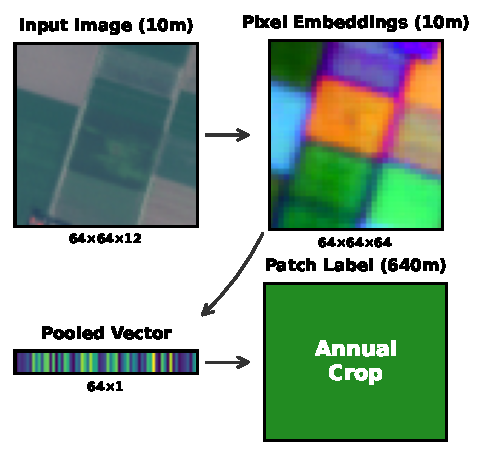
\includegraphics[width=\linewidth]{../paper/figures/hero.pdf}
  \end{columns}
\end{frame}

\begin{frame}{Pooling matters in other domains}
  \vspace{0.5em}
  \begin{columns}[T]
    \column{0.3\textwidth}
    \centering
    \textbf{Image Retrieval}\\[6pt]
    GeM pooling consistently\\
    outperforms mean pooling\\[6pt]
    {\footnotesize Radenovi\'{c} et al., 2018}

    \column{0.3\textwidth}
    \centering
    \textbf{Audio / Video}\\[6pt]
    Stats pooling (mean+std)\\
    summarizes variable-length\\
    sequences effectively\\[6pt]
    {\footnotesize Miech et al., 2017}

    \column{0.3\textwidth}
    \centering
    \textbf{Object-Based IA}\\[6pt]
    Bag of Visual Words\\
    uses region histograms\\
    for classification\\[6pt]
    {\footnotesize Csurka et al., 2004}
  \end{columns}

  \vspace{1.5em}
  \centering
  Yet pooling is \alert{largely unexplored} for earth embeddings.
\end{frame}

% ==========================================================
\section{EuroSAT-Embed}
% ==========================================================

\begin{frame}{EuroSAT-Embed: a pooling research benchmark}
  81,000 pixel-embedding GeoTIFFs from three foundation models,\\
  aligned to EuroSAT (27k patches, 10 land-cover classes).

  \vspace{0.8em}
  \begin{columns}[c]
    \column{0.3\textwidth}
    \centering
    \textbf{AlphaEarth}\\
    64-d, \texttt{int8}, 3.3\,GB

    \column{0.3\textwidth}
    \centering
    \textbf{OlmoEarth-Nano}\\
    128-d, \texttt{float32}, 40\,GB

    \column{0.3\textwidth}
    \centering
    \textbf{Tessera}\\
    512-d, \texttt{float32}, 164\,GB
  \end{columns}

  \vspace{0.8em}
  Reproducible pooling research \textbf{without re-running}
  expensive GFM inference.

  \vspace{0.5em}
  Evaluated on \textbf{random} (i.i.d.)
  and \textbf{spatial} (geographically disjoint) splits.

  \vspace{0.5em}
  {\footnotesize
    \texttt{CC-BY-4.0} \quad
    \url{https://hf.co/datasets/isaaccorley/eurosat-embed}}
\end{frame}

% ==========================================================
\section{Pooling Methods}
% ==========================================================

\begin{frame}{First-order pooling}
  Given $X \in \mathbb{R}^{H \times W \times D}$ with $N = HW$ pixels:

  \vspace{0.8em}
  \begin{columns}[T]
    \column{0.45\textwidth}
    \textbf{Mean} (baseline)
    $$\mu = \frac{1}{N}\sum_i x_i$$

    \textbf{Max} --- per-channel maximum

    \column{0.45\textwidth}
    \textbf{Generalized Mean (GeM)}
    $$\text{GeM}_p = \left(\frac{1}{N}\sum_i x_i^{\,p}\right)^{\!1/p}$$

    \textbf{Center-weighted mean} --- Gaussian kernel
  \end{columns}

  \vspace{1em}
  All preserve original dimensionality ($1\!\times$).
\end{frame}

\begin{frame}{Distributional and parametric pooling}
  \textbf{Hypothesis:} class signal lives in the \emph{distribution},
  not just the mean.

  \vspace{0.8em}
  \begin{columns}[T]
    \column{0.45\textwidth}
    \textbf{Distributional (training-free):}
    \begin{itemize}
      \item Mean+Std, Mean+Max ($2\!\times$)
      \item Median+IQR ($2\!\times$)
      \item Stats [min/max/$\mu$/$\sigma$] ($4\!\times$)
      \item Percentiles [10..90] ($5\!\times$)
      \item Covariance upper-tri
    \end{itemize}

    \column{0.45\textwidth}
    \textbf{Parametric (need training data):}
    \begin{itemize}
      \item PCA --- project to lower dim
      \item BoVW --- $k$-means histogram
    \end{itemize}

    \vspace{0.8em}
    E.g., a residential patch and an industrial
    area can share a mean but differ wildly
    in variance.
  \end{columns}
\end{frame}

% ==========================================================
\section{Setup}
% ==========================================================

\begin{frame}{Evaluation protocol}
  \vspace{0.5em}
  \centering
  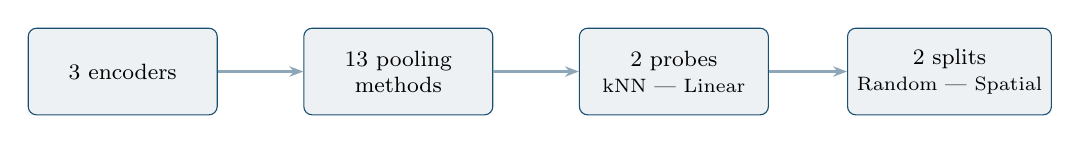
\begin{tikzpicture}[
    box/.style={draw=ocean, fill=ocean!8, rounded corners=3pt,
                minimum width=2.4cm, minimum height=1.1cm,
                align=center, font=\footnotesize},
    arr/.style={-{Stealth[length=5pt]}, thick, ocean!50}
  ]
    \node[box] (enc) at (0, 0) {3 encoders};
    \node[box] (pool) at (3.5, 0) {13 pooling\\methods};
    \node[box] (probe) at (7, 0) {2 probes\\{\scriptsize kNN | Linear}};
    \node[box] (split) at (10.5, 0) {2 splits\\{\scriptsize Random | Spatial}};

    \draw[arr] (enc) -- (pool);
    \draw[arr] (pool) -- (probe);
    \draw[arr] (probe) -- (split);
  \end{tikzpicture}

  \vspace{0.4em}
  {\large \textbf{= 156 experiments}}

  \vspace{1em}
  \begin{columns}[T]
    \column{0.45\textwidth}
    \textbf{kNN} ($k{=}5$, cosine distance)\\
    Probes geometric / similarity structure

    \column{0.45\textwidth}
    \textbf{Linear} (logistic regression, L-BFGS)\\
    Probes linear separability
  \end{columns}
\end{frame}

% ==========================================================
\section{Results}
% ==========================================================

\begin{frame}{Distributional statistics improve generalization}
  \begin{columns}[c]
    \column{0.48\textwidth}
    Linear probe on \textbf{spatial} splits:

    \vspace{0.5em}
    \renewcommand{\arraystretch}{1.3}
    \begin{tabular}{lr}
      Mean (baseline) & 76--84\% \\
      Mean+Max & 87--89\% \\
      \textbf{Stats} & \textbf{88--91\%} \\
    \end{tabular}

    \vspace{0.6em}
    \alert{+7--10\%} gain over mean pooling.

    \vspace{0.5em}
    On random splits, differences shrink
    to 3--5\% (spatial leakage flatters everyone).

    \vspace{0.5em}
    The spatial split is the honest evaluation.

    \column{0.48\textwidth}
    \centering
    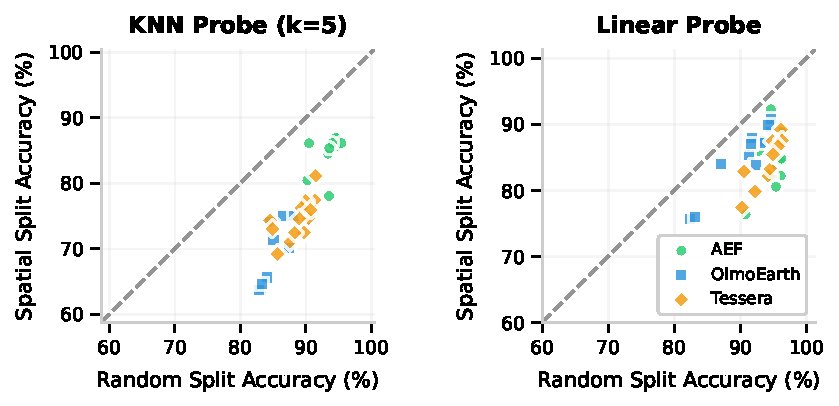
\includegraphics[width=\linewidth]{../paper/figures/random_vs_spatial.pdf}

    {\footnotesize Closer to diagonal = smaller gap}
  \end{columns}
\end{frame}

\begin{frame}{GeM: zero-cost upgrade}
  \begin{columns}[c]
    \column{0.5\textwidth}
    \textbf{Generalized Mean} ($p{=}3$):
    $$\text{GeM} = \left(\frac{1}{N}\sum_i x_i^{\,3}\right)^{\!1/3}$$

    \begin{itemize}
      \item \alert{+5\% spatial accuracy} over mean
      \item Same dimensionality ($1\!\times$)
      \item No training, no storage overhead
      \item Consistent across all three encoders
    \end{itemize}

    \vspace{0.5em}
    Softly upweights high-activation pixels without
    the harsh cutoff of max pooling.

    \column{0.45\textwidth}
    \centering
    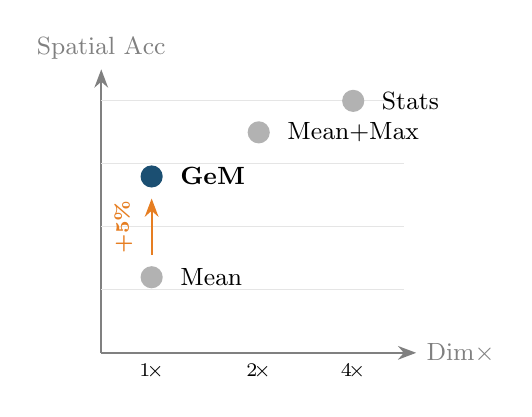
\begin{tikzpicture}[scale=0.8]
      \draw[-{Stealth}, thick, gray] (0,0) -- (5,0)
        node[right, font=\small] {Dim$\times$};
      \draw[-{Stealth}, thick, gray] (0,0) -- (0,4.5)
        node[above, font=\small] {Spatial Acc};
      \foreach \y in {1,2,3,4}
        \draw[gray!20] (0,\y) -- (4.8,\y);

      \fill[gray!60] (0.8, 1.2) circle (5pt);
      \node[right, font=\small] at (1.1, 1.2) {Mean};

      \fill[ocean] (0.8, 2.8) circle (5pt);
      \node[right, font=\small\bfseries] at (1.1, 2.8) {GeM};

      \fill[gray!60] (2.5, 3.5) circle (5pt);
      \node[right, font=\small] at (2.8, 3.5) {Mean+Max};

      \fill[gray!60] (4.0, 4.0) circle (5pt);
      \node[right, font=\small] at (4.3, 4.0) {Stats};

      \node[font=\scriptsize] at (0.8, -0.3) {$1\!\times$};
      \node[font=\scriptsize] at (2.5, -0.3) {$2\!\times$};
      \node[font=\scriptsize] at (4.0, -0.3) {$4\!\times$};

      \draw[-{Stealth}, thick, accent]
        (0.8, 1.55) -- (0.8, 2.45);
      \node[font=\scriptsize\bfseries, accent, rotate=90]
        at (0.35, 2.0) {+5\%};
    \end{tikzpicture}
  \end{columns}
\end{frame}

\begin{frame}{Accuracy--dimensionality tradeoff}
  \centering
  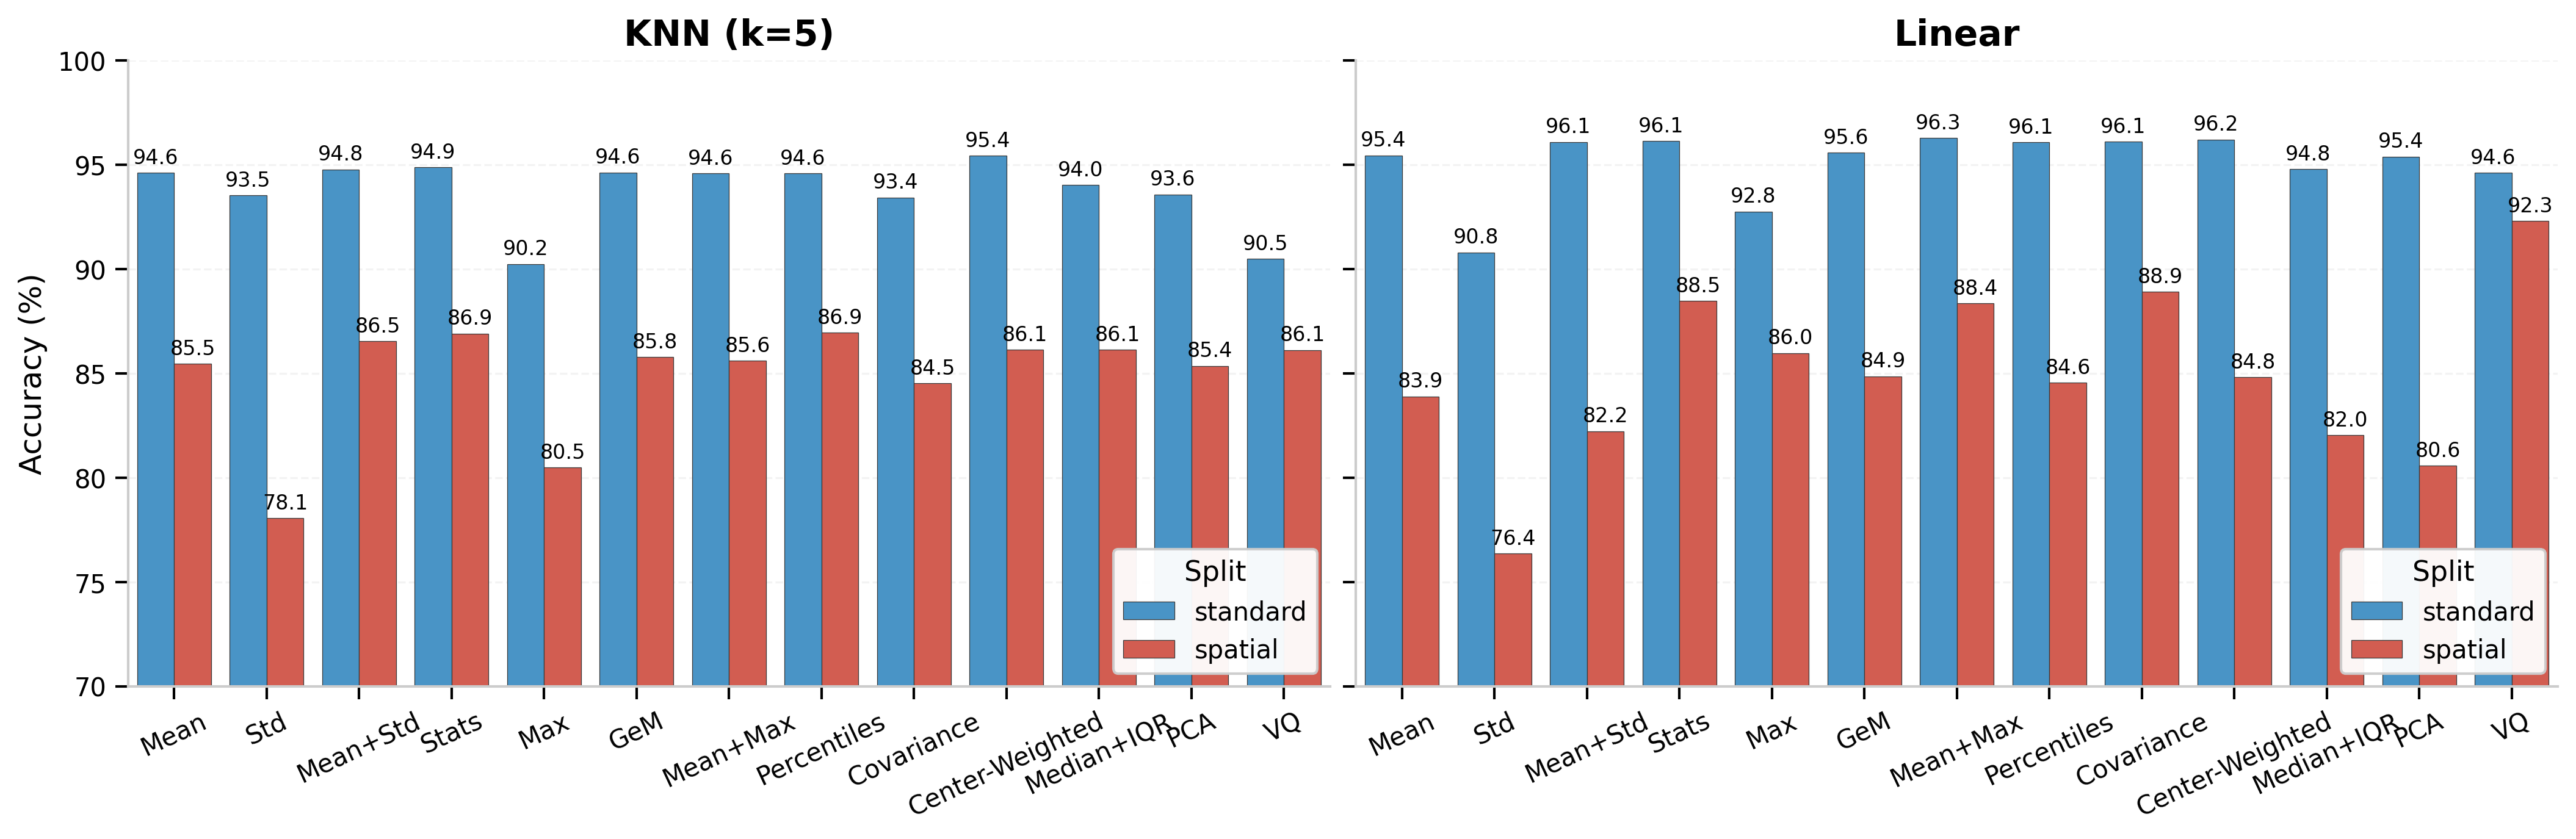
\includegraphics[width=0.6\linewidth]{../paper/figures/performance_comparison.png}

  \vspace{0.8em}
  \begin{columns}[c]
    \column{0.3\textwidth}
    \centering
    \textbf{No overhead ($1\!\times$)}\\
    GeM (+5\%)

    \column{0.3\textwidth}
    \centering
    \textbf{Best tradeoff ($2\!\times$)}\\
    Mean+Max (+6--8\%)

    \column{0.3\textwidth}
    \centering
    \textbf{Peak accuracy ($4\!\times$)}\\
    Stats (+7--10\%)
  \end{columns}
\end{frame}

\begin{frame}{Pooling interacts with the encoder}
  \begin{columns}[T]
    \column{0.3\textwidth}
    \textbf{AlphaEarth} {\small (64-d)}

    \vspace{0.3em}
    BoVW hits 92.3\% (linear) but
    fails on other encoders.

    \vspace{0.3em}
    Compact embeddings are naturally
    more robust to shift.

    \column{0.3\textwidth}
    \textbf{OlmoEarth} {\small (128-d)}

    \vspace{0.3em}
    Std alone boosts kNN by
    +11\% over mean.

    \vspace{0.3em}
    Second-order stats help similarity
    search more than linear probes.

    \column{0.3\textwidth}
    \textbf{Tessera} {\small (512-d)}

    \vspace{0.3em}
    Covariance pooling excels at kNN.

    \vspace{0.3em}
    Largest mean-pooling gap (12\%).
    High-dim benefits most from stats.
  \end{columns}

  \vspace{1em}
  \centering
  Higher embedding dimension $\Longrightarrow$
  more benefit from distributional statistics.
\end{frame}

\begin{frame}{Richer statistics close the generalization gap}
  \begin{columns}[c]
    \column{0.48\textwidth}
    \centering
    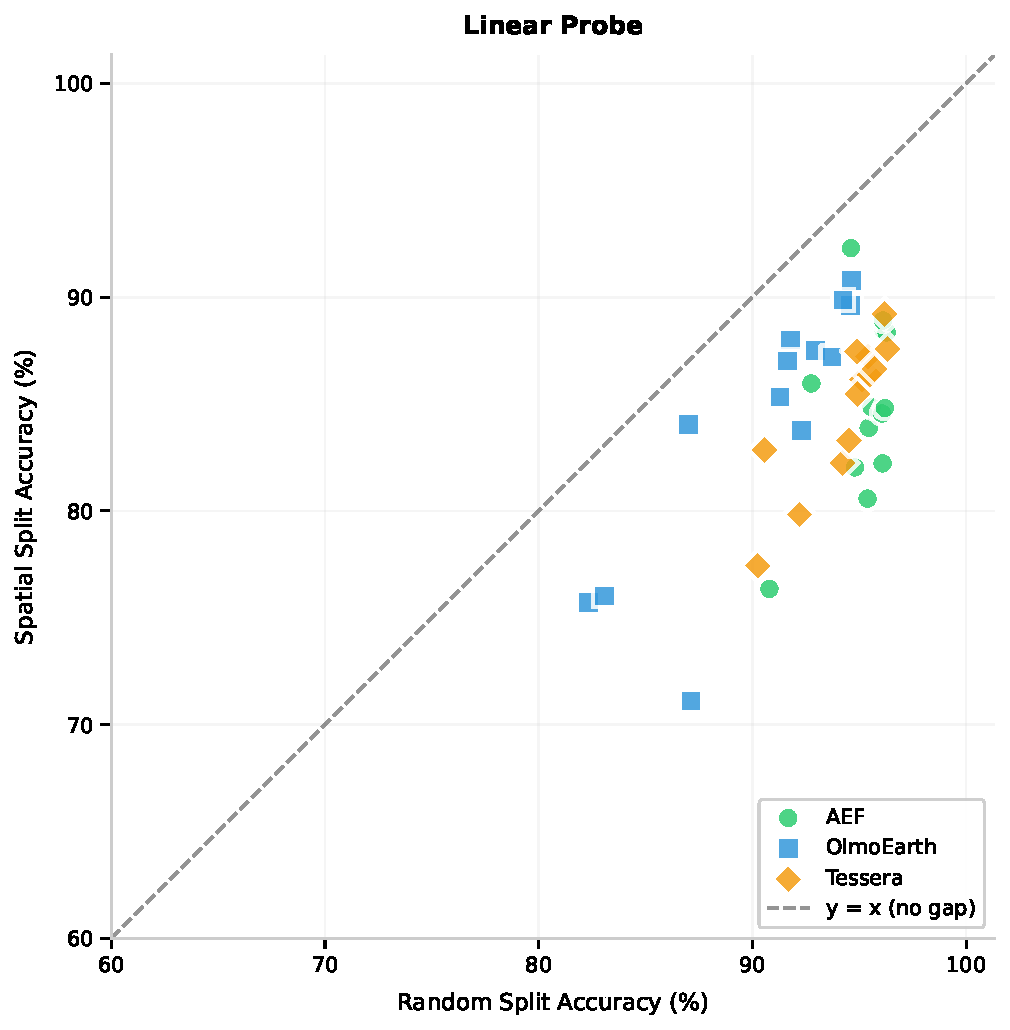
\includegraphics[width=\linewidth]{../paper/figures/random_vs_spatial_linear.pdf}

    \column{0.48\textwidth}
    Accuracy drop (random $\to$ spatial):

    \vspace{0.6em}
    \renewcommand{\arraystretch}{1.4}
    \begin{tabular}{lr}
      Mean & \textbf{10\%} drop \\
      Mean+Max & 6.4\% drop \\
      Stats & 6.2\% drop \\
      Max & 5.8\% drop \\
    \end{tabular}

    \vspace{0.8em}
    Mean pooling discards intra-patch
    heterogeneity that matters most
    under geographic shift.
  \end{columns}
\end{frame}

% ==========================================================
\section{Takeaways}
% ==========================================================

\begin{frame}{Recommendations}
  \centering
  \vspace{0.3em}
  \renewcommand{\arraystretch}{1.35}
  \begin{tabular}{llcc}
    \toprule
    \textbf{Scenario} & \textbf{Method} & \textbf{Gain} & \textbf{Dim} \\
    \midrule
    Drop-in default & GeM ($p{=}3$) & +5\% & $1\!\times$ \\
    Best accuracy & Stats [min/max/$\mu$/$\sigma$] & +7--10\% & $4\!\times$ \\
    Balanced & Mean+Max & +6--8\% & $2\!\times$ \\
    kNN retrieval & Covariance / Percentiles & +3--7\% & varies \\
    \bottomrule
  \end{tabular}

  \vspace{1em}
  All recommended methods are \textbf{training-free}
  and consistent across encoders.

  \vspace{0.5em}
  Start with GeM. Upgrade to Stats if you can
  afford $4\!\times$ the storage.
\end{frame}

\begin{frame}{Why does this work?}
  \begin{columns}[T]
    \column{0.45\textwidth}
    \textbf{The intuition}

    \vspace{0.3em}
    Mean pooling collapses a patch into
    a single ``average pixel.''

    \vspace{0.3em}
    A residential neighborhood and an
    industrial park can share a similar mean
    but differ in variance --- mixed rooftops,
    roads, vegetation vs.\ uniform warehouses.

    \vspace{0.3em}
    Higher-order statistics preserve
    that heterogeneity.

    \column{0.45\textwidth}
    \textbf{Broader implications}

    \vspace{0.3em}
    Extends GeM results from image retrieval
    to the geospatial domain.

    \vspace{0.3em}
    Foundation models encode fine-grained
    semantic structure worth preserving.

    \vspace{0.3em}
    Aggregation should be a design decision,
    not an afterthought.
  \end{columns}
\end{frame}

\begin{frame}{Limitations \& future directions}
  \begin{columns}[T]
    \column{0.45\textwidth}
    \textbf{Limitations}
    \begin{itemize}
      \item Single benchmark (EuroSAT)
      \item Three embedding sources
      \item Fixed hyperparameters
    \end{itemize}

    \column{0.45\textwidth}
    \textbf{Next steps}
    \begin{itemize}
      \item BigEarthNet, fMoW
      \item Learned / attention pooling
      \item Temporal aggregation
    \end{itemize}
  \end{columns}

  \vspace{1.2em}
  \centering
  \textbf{Open resources}\\[4pt]
  {\small
    Dataset: \url{https://hf.co/datasets/isaaccorley/eurosat-embed}\\[3pt]
    Code: \url{https://github.com/isaaccorley/geopool}}
\end{frame}

% ==========================================================
\begin{frame}[standout]
  Questions?

  \vspace{1.5em}
  \begin{columns}[c]
    \column{0.4\textwidth}
    \centering
    
\includegraphics[width=4.5cm]{qr_code.png}\\[6pt]
    {\small Code}

    \column{0.4\textwidth}
    \centering
    
\includegraphics[width=4.5cm]{qr_data.png}\\[6pt]
    {\small Dataset}
  \end{columns}
\end{frame}

\end{document}
